\section*{Osazování}

Osazování je nejlepší provádět od nejmenších součástek po ty největší. Je tedy vhodné napřed osadit LED diody v pouzdře 0603, poté rezistory a kondenzátory v pouzdrech 0805. Následně mikrokontrolér v pouzdře SO-8 a nakonec tlačítko. Vypínač je vhodné přiletovat až když je kostka smontovaná, tak aby dobře pasoval do předchystaného otvoru.

Pozor na správnou polarizaci LED diod! Dioda je polarizovaná součástka, která má anodu a katodu. Katoda je označena malým kolečkem s horní strany a zelenou značkou ze strany spodní. Pokud budou diody nesprávně otočeny nebudou svítit. Správně otočit je třeba i mikrokontrolér, který při nevhodném otočení shoří. na osazovacím plánu je jednička mikrokontroléru označena čárkou. Poslední věcí, na kterou je třeba dávat obzvláště pozor je správné otočení baterie. Kladný pól, ten větší na kterém je napsáno obvykle +, musí být položen na velkou plošku, sodní destička, na které nejsou součástky. Záporný pól, ten menší je třeba připojit k malé plošce, která je na straně součástek na hlavní destičce. Při špatném otočení baterie je kostka zničena! Tak hodně štěstí.

\begin{figure}[H]
  \centering
  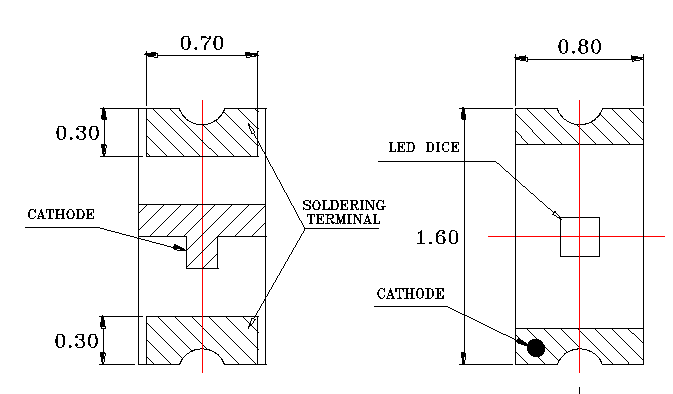
\includegraphics[width=\textwidth]{../img/LED.pdf}
  \caption{Označení katody}
  \label{img:1}
\end{figure}